\chapter{Prototypen Bau}\label{chap:Prototypen_Bau}
Nachdem in den vorherigen Kapiteln die Implementierung der Software beschrieben wurde, wird in diesem Kapitel die Vorgehensweise bei dem Bau des Prototypen, inklusive Bau selbst, vorgestellt. Um die Funktionalität des Handspiegels sicher zu stellen müssen einige Bedingungen bei dem Bau des Prototypen beachtet werden (siehe Abbildung \ref{fig:protoyp_skizze_ori}).
\begin{figure}[h]
	\centering
	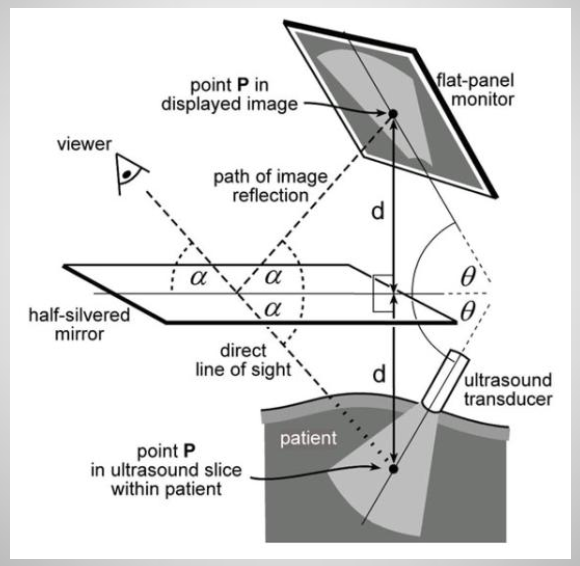
\includegraphics[width=0.95\textwidth]{Prototypen_Bau/Sketch1}
	\caption{Originale Skizze des Prototypen}
	\label{fig:protoyp_skizze_ori}
	%SOURCE Image Source: G. Stetten et al. "Towards a clinically useful Sonic Flashlight," %IEEE International Symposium
%on Biomedical Imaging 2002 
\end{figure}
In der Abbildung sieht man wie Ultraschallsonde, Smartphone und halb-durchlässiger Spiegel zueinander angeordnet sein müssen, damit der optische Effekt (siehe Kapitel \ref{chap:Einleitung}) des Handspiegels erzeugt wird.\\
Der Winkel $\theta$ beschreibt den Winkel zwischen Smartphone und Teilerspiegel sowie zwischen Teilerspiegel und Ultraschallsonde. Wichtig dabei ist, dass der Winkel bei beiden gleich ist. Bei der Umsetzung ist zu beachten, dass die Winkel $\theta$ zwischen den Komponenten identisch sind und der Abstand eines Punktes P auf dem Display den selben Abstand zum Teilerspiegel besitzt, wie der  Teilerspiegel zum projiziertem Punkt P'. Das heißt ein Punkt \textit{x} auf dem Smartphone hat einen bestimmten Abstand \textit{d1} zu dem halb-durchlässigen Spiegel. Da der Punkt \textit{x} über den Spiegel optisch \textbf{in} den Körper projiziert wird, muss der Abstand zwischen dem reflektierten Punkt \textit{x} in dem Körper und dem Spiegel, dem Abstand \textit{d1} entsprechen.\\
Wird dieser Abstand \textit{d} nicht berücksichtigt, werden die Punkte an die falsche Stelle im Körper projiziert. Das bedeutet, dass eine Halsschlagader entweder zu tief oder zu flach im Körper gesehen wird, anstelle der wirklichen Position der Halsschlagader. Das gleiche passiert wenn $\theta$ ungleich ist. Falls der Winkel zwischen Smartphone und Spiegel größer ist, wird der Punkt tiefer in dem Körper abgebildet. Andersrum wird der Punkt näher an der Hautoberfläche abgebildet, wenn $\theta$ kleiner ist zwischen Smartphone und Spiegel.\\
Abgesehen von den genannten Anforderungen kommen noch weitere Anforderungen an den Prototypen, eine davon ist die Praktikabilität. Der Prototyp darf nicht zu schwer sein um einen Patienten über eine gewisse Zeit zu schallen, oder zu schwer um feine Bewegungen mit der Sonde auszuführen. Des Weiteren darf der behandelnde Arzt in seinen Bewegungen nicht eingeschränkt sein durch die Größe des Prototypen. Deswegen muss dieser so klein, handlich und leicht wie möglich gestaltet sein. Gleichzeitig muss der Prototyp stabil genug sein um bei einigen Behandlungen getestet zu werden. Zum Schluss muss beachtet werden, dass der Prototyp starr ist, also keine Bewegungsfreiheit hat. Er darf bei der Benutzung nicht wackeln oder seine Form verändern, damit er überhaupt benutzbar ist (siehe \ref{AnfAnalyse}).

\section{Materialienauswahl}
Um den Prototypen abbildungsgetreu zu bauen, kommen verschiedene Materialien und Möglichkeiten in Frage. Eine davon ist die genauen Maße der Sonde, des Smartphones und des Spiegels zu messen und abhängig davon ein 3D Modell im Computer zu modellieren. Dieses 3D Modell kann über einen 3D Drucker ausgedruckt werden und gegebenenfalls mit Klebe o.ä. an den Komponenten befestigt werden. Diese Möglichkeit verspricht die beste Qualität des Prototypen in Bezug auf die Robustheit, Praktikabilität und Einhaltung der in Kapitel \ref{chap:Prototypen_Bau} genannten Bedingungen. Neben der Vorteilen, besitzt dieser Ansatz aber auch Nachteile. Der ausschlaggebendste Nachtteil ist der enorme Einarbeitungsaufwand in die 3D Modellierung, dieser kann im zeitlichen Rahmen des Projektes nicht aufgebracht werden.\\
Der gewählte Ansatz kombiniert eine Reihe von verschiedenen Materialien. Dazu gehören Knete, Heißkleber, Kabelbinder, Winkelschrauben und eine Hülle für das Smartphone. Zusammen erfüllen diese Materialien die Anforderungen an den Prototypen, denn sie sind leicht und robust.

\section{Realisierung des Prototypen}

Bevor der Prototyp physikalisch gebaut werden kann, muss zuerst festgelegt werden wie der Prototyp aussehen soll. Dazu wird eine einfache Skizze entworfen, die alle nötigen Komponenten enthält und aufzeigt wie der Prototyp aussehen soll (siehe Abbildung \ref{fig:protoyp_skizze_umsetzung}).
\begin{figure}[h]
	\centering
	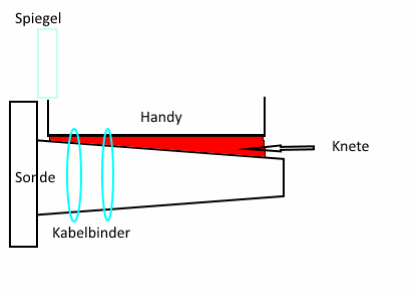
\includegraphics[width=0.80\textwidth]{Prototypen_Bau/Prototyp_skizze}
	\caption{Skizze der Umsetzung des Prototypen}
	\label{fig:protoyp_skizze_umsetzung}
\end{figure}
Die Abbildung zeigt wie die Materialien angebracht werden müssen um den gewünschten Prototypen zu bauen. Um die Skizze einfach zu halten sind nicht alle nötigten Komponenten eingezeichnet, wie zum Beispiel die Winkelschrauben. Im folgenden Abschnitt wird erklärt wie die Komponenten zusammen gebaut werden und warum sie so angeordnet sind.\\
Damit das Smartphone an der Sonde befestigt werden kann wird zuerst eine ebene Fläche benötigt. Dazu wird die unebene Oberfläche der Sonde mit einer Schicht Knete eben gezogen. Danach werden Löcher in die Handyhülle geschnitten, um diese mit Kabelbindern an der Sonde zu befestigen. Nun wird die Handyhülle auf die mit Knete geebnete Oberfläche der Sonde gedrückt und mit den Kabelbindern an der Sonde befestigt. Da die Handyhülle durch die Kabelbinder fest in die Knete gedrückt wird, ist diese stabil an der Sonde befestigt ohne einen Bewegungsspielraum zuzulassen. Anschließen werden zwei Winkelschrauben an dem linken Rand der Handyhülle, mithilfe von Heißkleber, befestigt (siehe Abbildung \ref{fig:protoyp}). Diese sorgen für den nötigen Winkel zwischen Smartphone, Spiegel und Sonde. Wobei $\theta$ auf beiden Seiten 90° beträgt. Abschließend wird der halb-durchlässige Spiegel, ebenfalls mithilfe von Heißkleber, an den Winkelschrauben befestigt.\\
\begin{figure}[h]
	\centering
	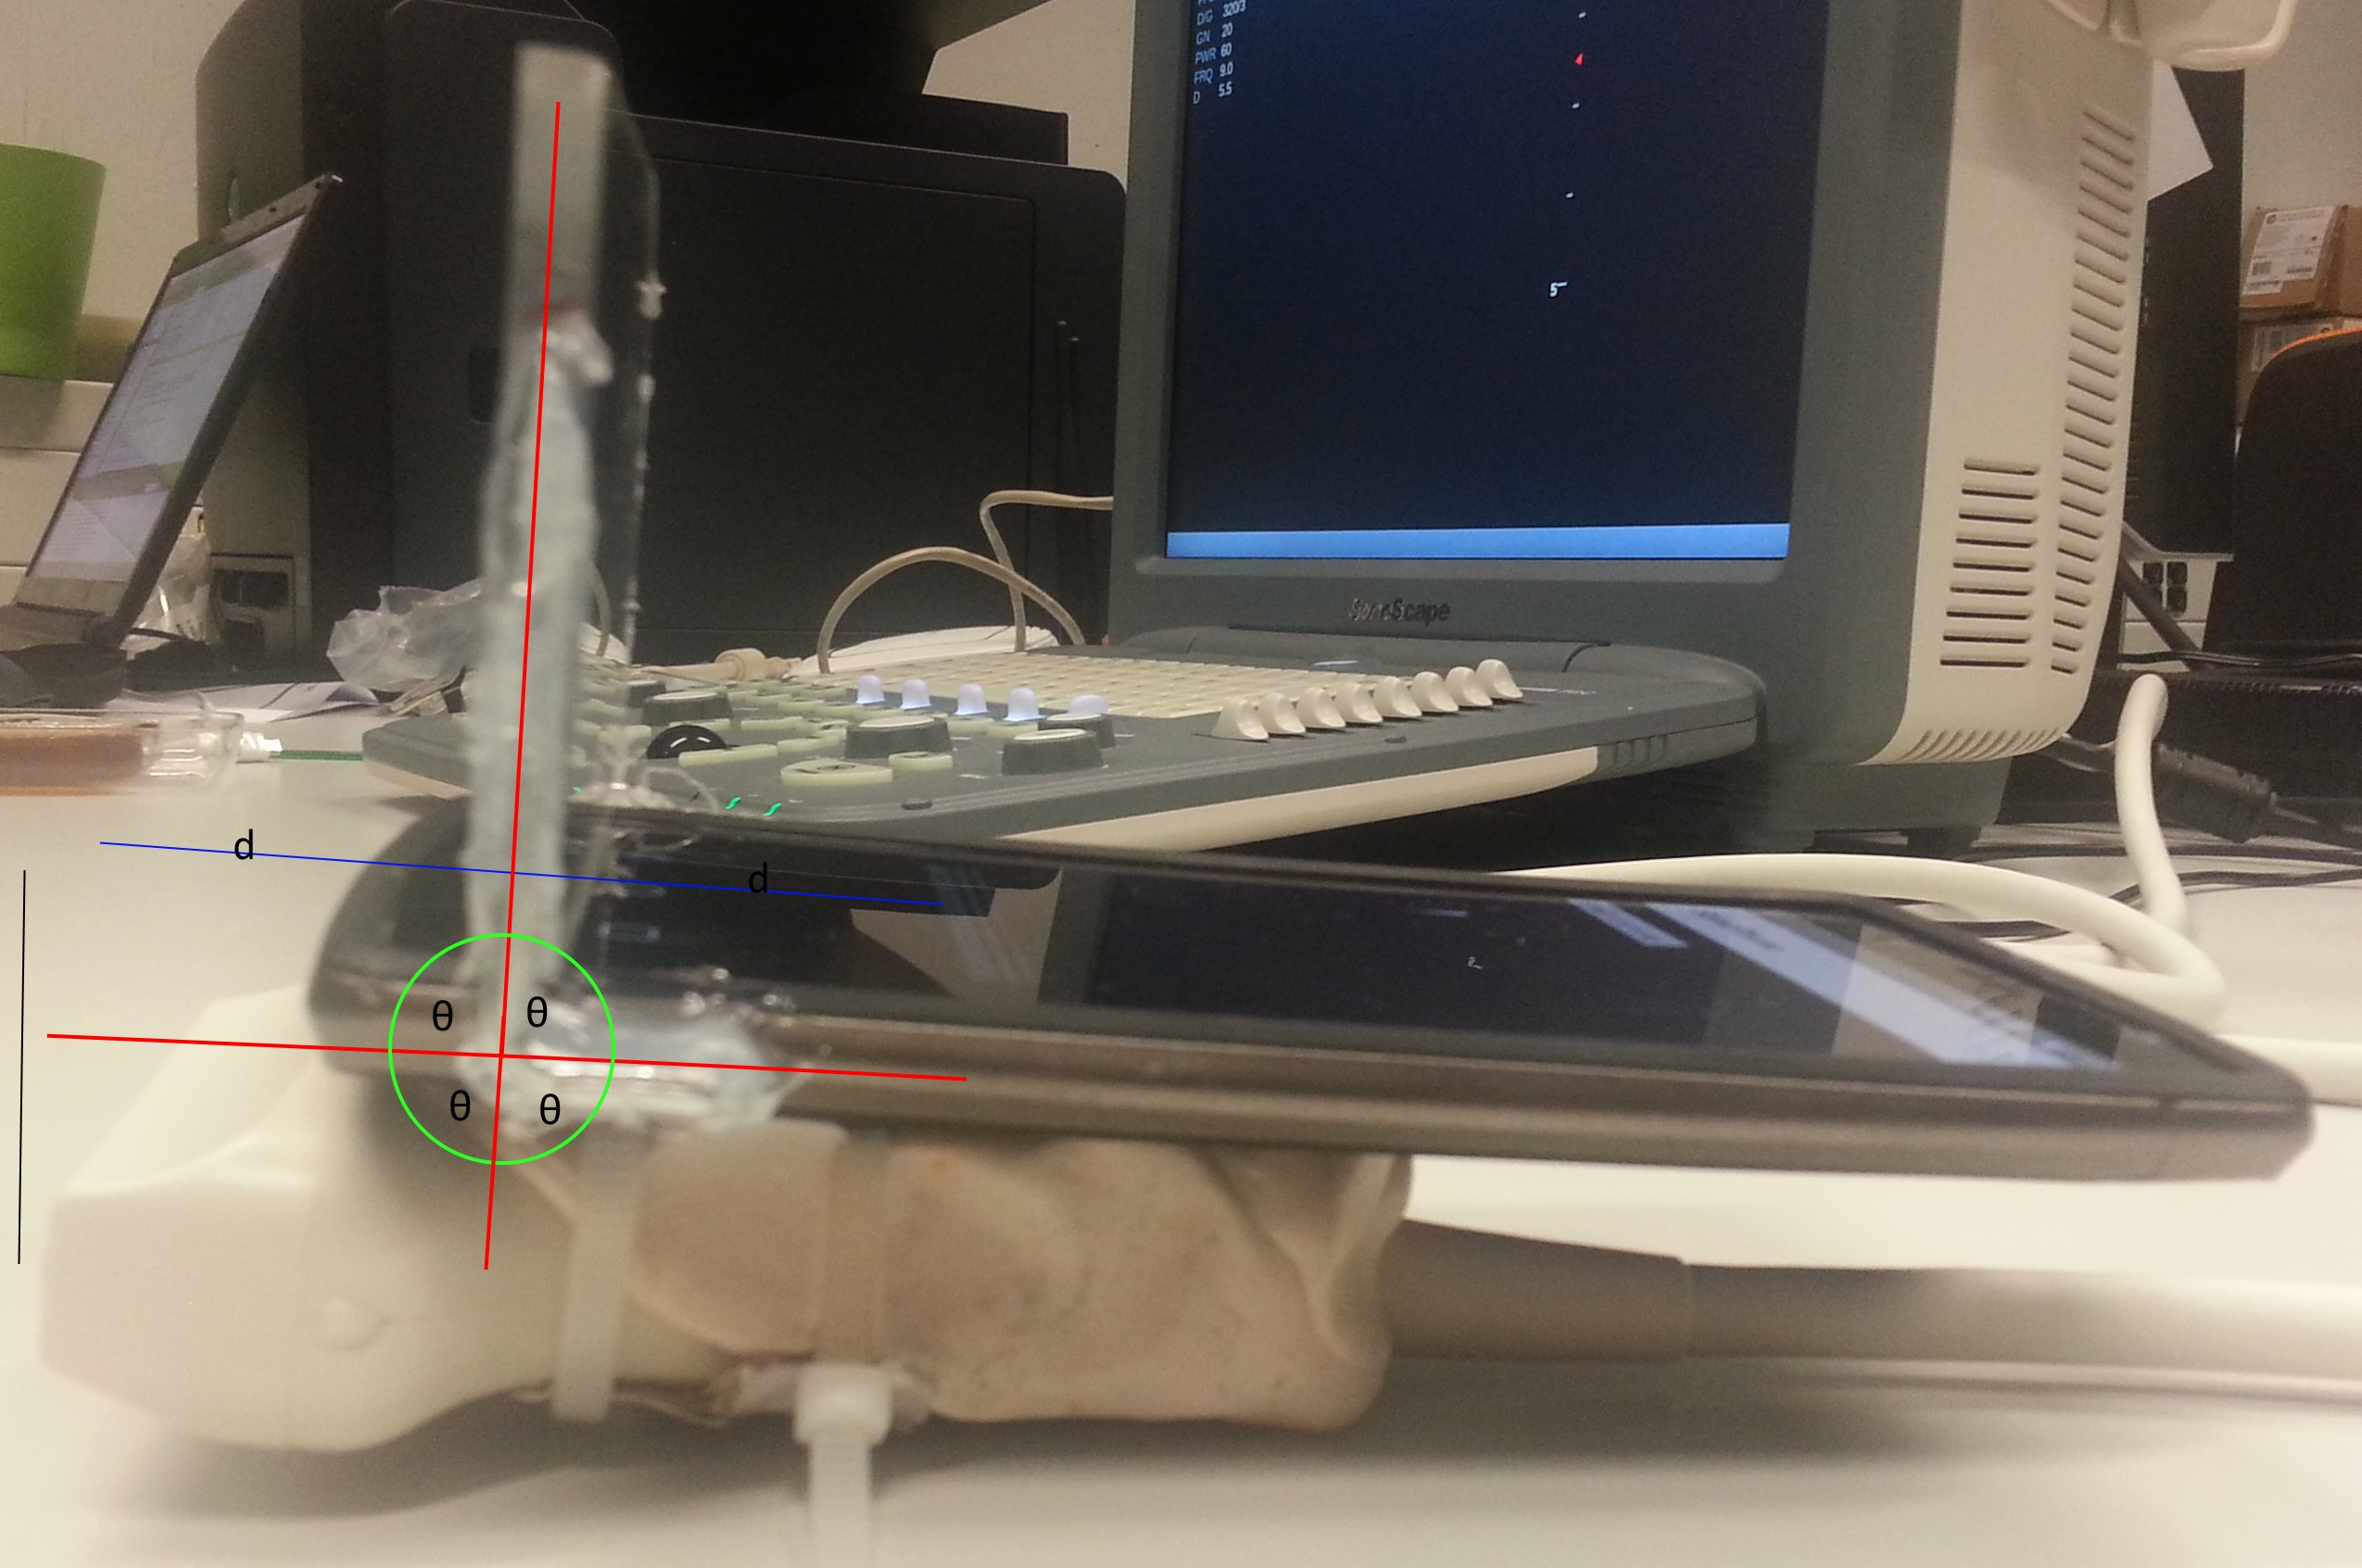
\includegraphics[width=0.98\textwidth]{Prototypen_Bau/Prototyp_fertig}
	\caption{Eigenschaften des fertigen Prototyps}
	\label{fig:protoyp}
\end{figure}
Der fertige Prototyp wird in Abbildung \ref{fig:protoyp} gezeigt. Auf der Abbildung sieht man, dass die Sonde unter dem Prototypen angebracht ist. Im Hintergrund ist das SonoScape Gerät im laufenden Betrieb zu erkennen, die Sonde mitsamt Prototyp ist also einsatzbereit. Zur Verdeutlichung der Einhaltung der Bedingungen aus Abbildung \ref{fig:protoyp_skizze_ori} sind zwei rote Strecken, eine blaue Strecke, eine schwarze Strecke und vier Winkel eingezeichnet. Da es sich um einen Prototypen handelt sind die Abstände und Winkel nicht einhundert Prozent genau, sondern so genau, dass die Illusion zu erkennen ist. Die zwei roten Strecken sind nur eingezeichnet um $\theta$ einzeichnen zu können. Der Winkel $\theta$ ist circa 90°, da in der Skizze der Winkel zwischen Spiegel und Smartphone gleich dem Winkel zwischen Spiegel und Sonde sein muss. Die blaue Strecke zeigt den Abstand \textit{d} zwischen einem Punkt \textit{x} und dem Spiegel, sowie den Abstand zwischen Spiegel und der Projektion von \textit{x}. Der Abstand vom Spiegel zum Anfang der Sonde muss also gleich dem Anstand des Spiegels bis zum ersten Pixelpunkt auf dem Smartphone sein. Deswegen befindet sich das Bild auf dem Smartphone nicht ganz unten, sondern genau die Distanz \textit{d} weit vom Spiegel entfernt. Bei genauem Hinsehen kann auf dem Display an dem rechten Ende der blauen Strecke der Anfang des Ultraschallbildes erkannt werden. Auf der Höhe des linken Endes der blauen Strecke befindet sich, bei einer Ultraschalluntersuchung, die Oberfläche des Objektes zum Beispiel die Haut des Patienten.\\
\begin{wrapfigure}{l}{0.4\textwidth}
\centering
\includegraphics*[width =0.4\textwidth]{Prototypen_Bau/Horizontale_distanz}
\caption{{\small Horizontale Distanz der Projektion zur Aufnahme}}
\label{fig:horizontale_distanz}
\end{wrapfigure}
Der Nachteil an diesem Prototypen ist die horizontale Distanz zwischen dem Kopf der Sonde und dem Display des Smartphones, repräsentiert durch die schwarze Strecke am linken Rand des Bildes. Dieser Versatz kann mit dieser Sondenform nicht vermieden werden, da das Smartphone sonst viel weiter hinten (rechts auf Abbildung \ref{fig:protoyp}) angebracht sein müsste. Das würde allerdings die Anforderung der Praktikabilität und der Stabilität verletzen und ist deswegen nicht möglich. Dieser Abstand hat zur Folge, dass die Projektion nicht genau in der Körperschicht liegt aus der sie aufgenommen wurde (rote Aufnahme in Abbildung \ref{fig:horizontale_distanz}), sondern verschoben um die horizontale Distanz, also der schwarzen Strecke aus Abbildung \ref{fig:protoyp}. Die eigentliche Projektion liegt dementsprechend verschoben in der Haut (siehe Abbildung \ref{fig:horizontale_distanz}.  Allerdings wird dieser Effekt durch den Betrachtungswinkel des behandelnden Arztes verringert, denn der Spiegel ist bei der Untersuchung in die Richtung des Arztes gedreht. Das hat zur Folge, dass der Arzt von vorne auf die Projektion schaut, dadurch wird der Versatz optisch verringert.\\
Trotzdem wurde das Konzept korrekt umgesetzt und die Projektion der Schichtaufnahme in die Haut findet statt. Die Bedingungen aus Abbildung \ref{fig:protoyp_skizze_ori} wurden umgesetzt, sowie die Anforderungen aus Kapitel \ref{AnfAnalyse} eingehalten.\\ 
Abbildung \ref{fig:protoyp2} zeigt nochmal den fertigen Prototypen ohne eingezeichnete Strecken und Winkel.
\begin{figure}[h]
	\centering
	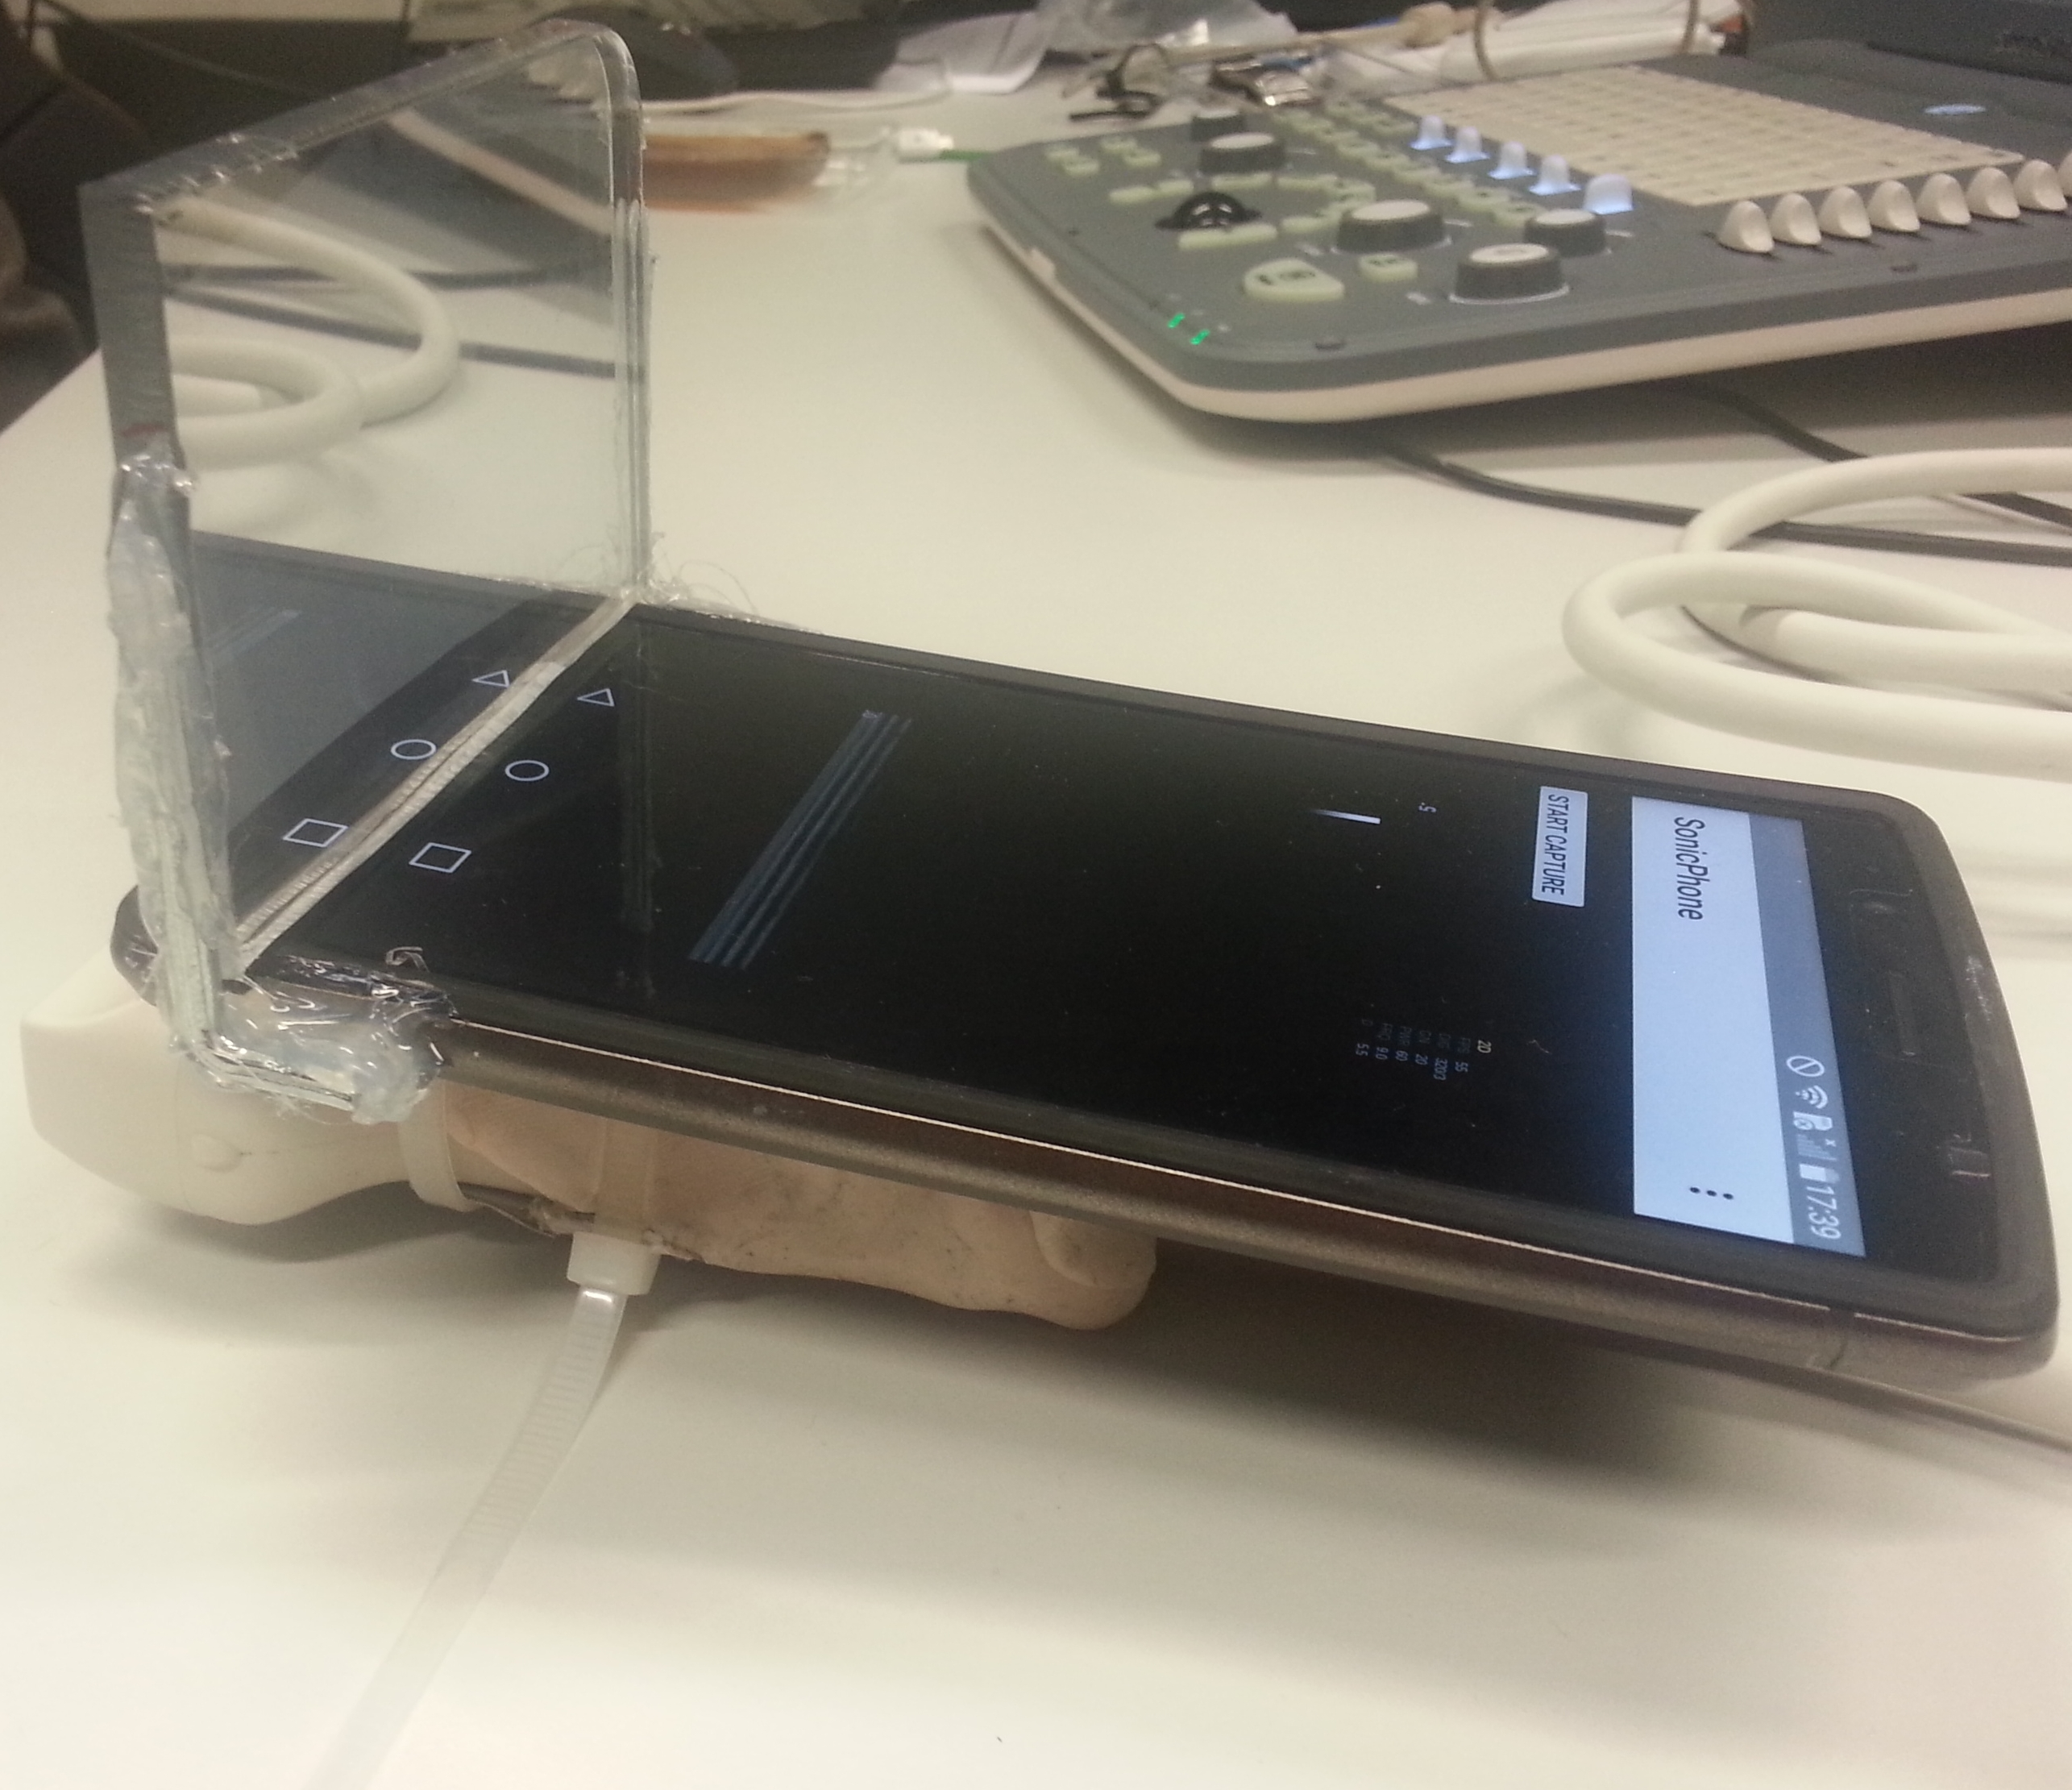
\includegraphics[width=0.98\textwidth]{Prototypen_Bau/Prototyp_fertig2}
	\caption{Prototyp}
	\label{fig:protoyp2}
\end{figure}



